%chapresult.tex
%
In this chapter, we will discuss the first measurement of the nucleon number $A$ and $Q^2$ dependence of nuclear transparency for the $A(e,e'K^+)$ process. Nuclear transparencies for $^{12}$C, $^{63}$Cu and $^{197}$Au nuclei over a  $Q^2$ range of 1.1 $\mathrm{to}$ 3.0 $(\mathrm{GeV/c})^2$ are shown with the super ratio of A$>$2 nuclei to deuterium.\footnote{Transparencies for these kinematic settings with the super ratio of A$>$1 nuclei to hydrogen are shown in APPENDIX \ref{Transparency with respect to Hydrogen}.} We also extracted average effective cross section for kaons in this kinematic range. We have compared our results with the available data to date.

%\Section{Cross sections}%
%Cross sections of Hydrogen target for three kinematics has been shown in \Tableref{t_1} and for all other targets have shown in \Tableref{t_2}.

\Section{Transparency}%
%
\label{Transparency}
The ratio of cross sections for exclusive processes from nuclei to those from nucleons is termed as Nuclear Transparency (T). The nuclear transparency was determined using the experimental charge-normalized yield, $\bar{Y}$ divided by the charge-normalized Monte Carlo equivalent yield, $\bar{Y}_{SIMC}$. For a given
target with nucleon number, A the nuclear transparency can be expressed as
\vspace{0.5in}
\begin{equation} \label{equ:nucltransp2}
T = 
\frac{\left(\bar Y/ \bar Y_{\rm MC} \right)_A}
{\left(\bar Y/ \bar Y_{\rm MC} \right)_{\rm D}},
\end{equation}

\noindent
where the denominator is the ratio of the yields for the deuterium target.
%\begin{center}$$T=\frac{\frac{\sigma_A^{Data}}{\sigma_A^{simc}}}{\frac{\sigma_0^{Data}}{\sigma_0^{simc}}}$$\end{center}

%\SubSection{Transparency with respect to Hydrogen}%
%\label{Transparency with respect to Hydrogen}
%Transparency of Kaon with respect to free nucleon cross section for three kinematics for all the targets has been shown in \Tableref{t_2}. We used Hydrogen cross section as free nucleon cross section. The total uncertinity has been taken as the qudrature sum of the statistical and systematic uncertinity. The differnt targets are shown by different colors as: black- $LD_2$, red- Carbon, green- Copper and blue- Gold for three different kinematics of $Q^2$= 1.1, 2.2 and 3.0 $(GeV/c)^2$. In the \figureref{transp1} the inner bar shows the statistical uncertinity and outer bar shows the systemetic uncertinity and total uncertinity as qudrature sum these two.


\SubSection{Transparency with Respect to Deuterium}%
Hydrogen consists of just one proton, and hence we considered its cross section as a free-nucleon cross section. But for all A$>$1 targets, we have neutrons. As deuterium has one proton and one neutron and one can produce ($K^+\Sigma^-$) from the neutron, therefore it is more appropriate to calculate transparency with respect to deuterium.\footnote{The transparencies with respect to the free-space cross section are shown in APPENDIX \ref{Transparency with respect to Hydrogen}.} Transparency of kaon with respect to $LD_2$ for three kinematics for all the targets are presented in \Tableref{t_4}. In \figureref{transp2} the variation of transparency with $Q^2$ is shown. Different targets are shown by different colors: (RED- Carbon, GREEN- Copper and BLUE- Gold) for the three different kinematic settings of $Q^2$= 1.1, 2.2 and 3.0 $(\mathrm{GeV/c})^2$. In \figureref{transp2}, the inner bar shows the statistical uncertainty and the outer bar shows the systematic uncertainty and total uncertainty as quadrature sum of these two.

\begin{table}
  \caption[T and $\sigma_{eff}$ for different targets with respect to $LD_2$.]{\label{tab:t_4}T and $\sigma_{eff}$ for different targets with respect to $LD_2$.}
\begin{center}
\begin{tabular}{||c|c|c|c|c|c|c||}\hline
 Target & $Q^2$ & Transparency & Statistical & Systematic & Total \\
 & $(GeV/c)^2$ & & error($\%$)& error($\%$)&error($\%$) \\\hline
Carbon & 1.1 & 0.90 &10.64 &16.11 &19.31\\
Copper & 1.1 & 1.06 &08.27 &10.83 &13.63\\
Gold   & 1.1 & 0.91 &11.63 &12.84 &17.32\\\hline
Carbon & 2.2 & 0.62 &09.39 &12.68 &15.78\\
Copper & 2.2 & 0.74 &07.24 &07.62 &10.52\\
Gold   & 2.2 & 0.79 &10.39 &13.65 &17.16\\\hline
Carbon & 3.0 & 0.43 &10.40 &07.13 &12.61\\
Copper & 3.0 & 0.60 &10.46 &07.60 &12.93\\
Gold   & 3.0 & 0.63 &14.03 &12.92 &19.07\\\hline
\end{tabular}
\end{center}
\end{table}
%\Table{t_4}{Transparency and cross section for different targets and of $Q^2$ for kaon with respect to the cross section of $LD_2$.}
%\begin{singlespace}
% Different kinematic settings for kaon with respect to the cross section of $LD_2$ are shown here.
%\end{singlespace}

\begin{figure}[!tbp]
  \centering
  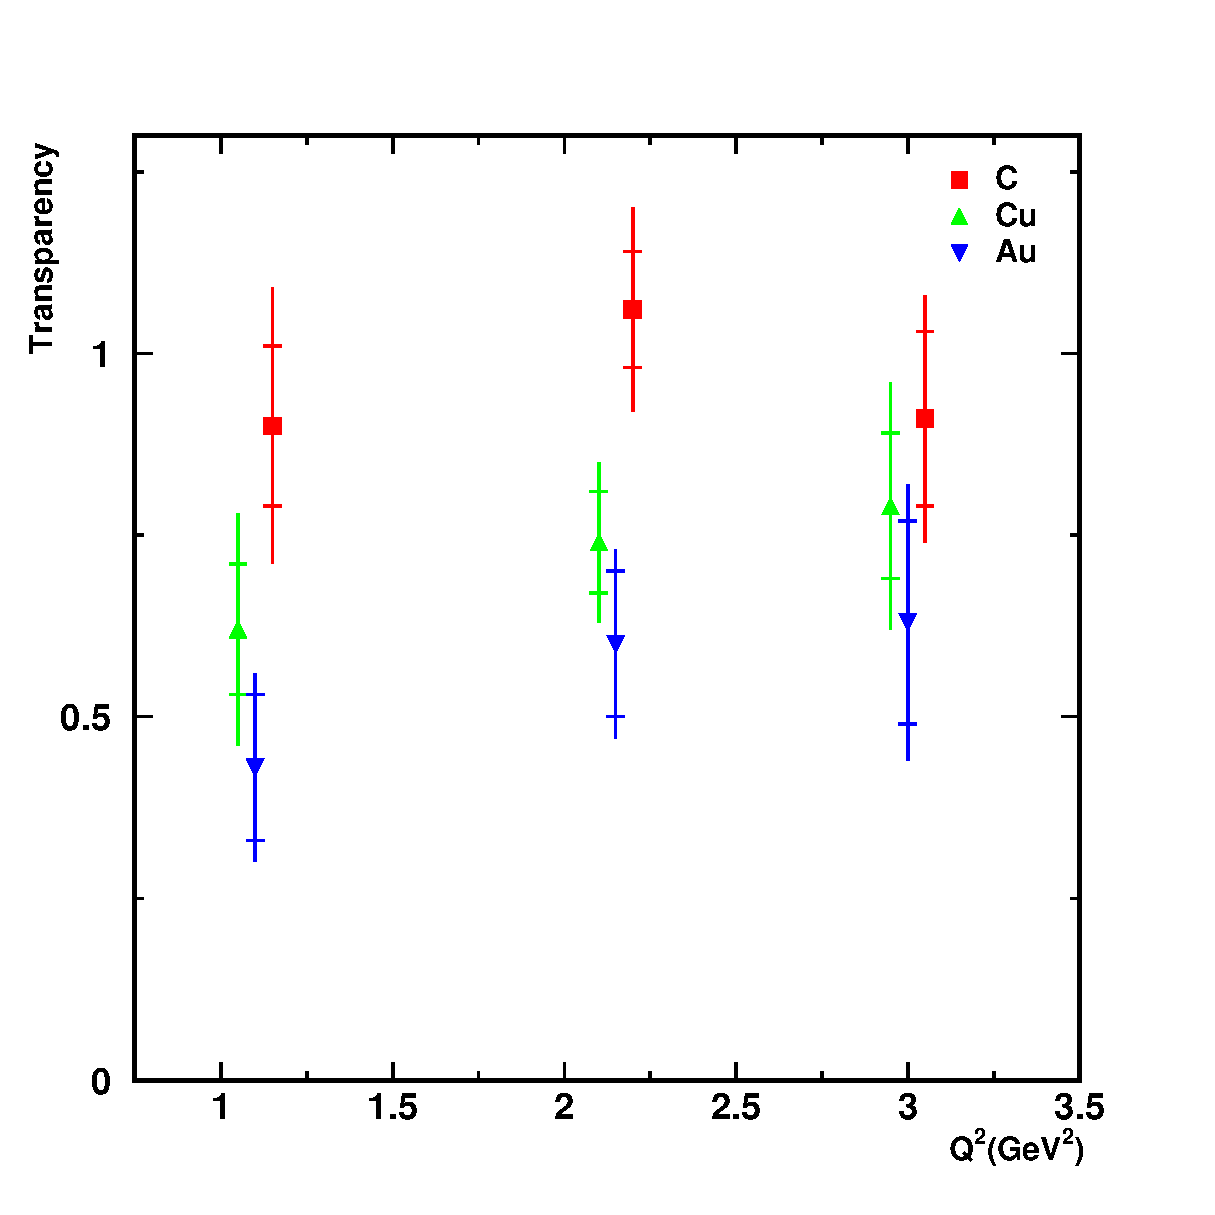
\includegraphics[width=0.8\columnwidth]{transp2}
  \caption[Nuclear transparency for targets of $A>$2 with respect to $LD_2$.]{\label{fig:transp2}Nuclear transparency for targets of $A>$2 with respect to $LD_2$.\\\\ Carbon and copper are shifted by 0.05 and -0.05 $(\mathrm{GeV/c})^2$ in $Q^2$, respectively, with respect to gold for convenience. The targets are shown in different colors as RED- carbon, GREEN- copper and BLUE- gold.}
\end{figure}
%\setlength{\figwidth}{0.8\linewidth}
%\Figure{transp2}{\figwidth}{Nuclear transparency for targets of $A>$2 with respect to $LD_2$. Carbon and copper are shifted by 0.05 and -0.05 $(\mathrm{GeV/c})^2$ in $Q^2$, respectively, with respect to gold for convenience. The targets are shown in different colors as \textcolor{red}{RED}- carbon, \textcolor{green}{GREEN}- copper and \textcolor{blue}{BLUE}- gold.}

%\Figure{alpha}{\figwidth}{$\alpha$ for differnt kinematics with theoritical band.}
%
\Section{Error Calculation}%
\label{Error Calculation}
In this section we briefly describe the error analysis for the statistical and systematic error in the experiment.

\SubSection{Statistical Error Calculation}%
\label{Statistical Error Calculation}
The statistical uncertainties in the charge-normalized experimental yields were calculated for each run and summed over the runs at a given kinematic setting. The total charge-normalized yield can be written as

\begin{equation} \label{equ:staterror1}
\bar{Y} = 
\left(\sum^{n}_{i}\frac{\bar{Y}_i}{(\bar{Y}_i/\sqrt{N_i})^2}\right)
\left(\sum^{n}_{i}\frac{1}{(\bar{Y}_i/\sqrt{N_i})^2}\right)^{-1}
\end{equation}

\noindent
where $i$ represents the $i^{th}$ run of a kinematic setting and $N_i$ is the number of events inside the experimental acceptance. The statistical uncertainty for the entire setting, $d\bar{Y}$ , can be written as

\begin{equation} \label{equ:staterror2}
d\bar{Y} = 
\left(\sum^{n}_{i}N_i/\bar{Y}_i^2\right)^{-\frac{1}{2}}
\end{equation}

We applied the same acceptance and missing mass cuts to both the experimental data and the Monte Carlo events. The Monte Carlo statistical error was determined in a similar fashion, except $N_i$ was replaced with the raw number of Monte Carlo particles that passed these cuts. Then statistical uncertainty in the transparency, $dT_{stat}$, was given by \cite{BC06}

\begin{equation} \label{equ:staterror3}
dT_{stat} = 
T \times \sqrt{\left(\left[d\bar{Y}/\bar{Y}\right]^2 + \left[d\bar{Y}_{SIMC}/\bar{Y}_{SIMC}\right]^2 \right)_A + 
\left(\left[d\bar{Y}/\bar{Y}\right]^2 + \left[d\bar{Y}_{SIMC}/\bar{Y}_{SIMC}\right]^2\right)_D}
\end{equation}

\SubSection{Systematic Error Calculation}%
\label{Systematic Error Calculation}
%We used same systemetic uncertinities from pion transparecy calculation \cite{BC06} except the uncertinities Particle ID and Cut Dependence. 
As we are using the same set of data from experiment E01-107 as used in pion transparency analysis, most of the uncertainties are same as determined during the  pion transparency analysis \cite{BC06}. The two uncertainties that differ are uncertainty in particle identification and cut dependence. An important aspect was to investigate the stability of the results as a function of the applied cuts. The cut dependence was calculated by measuring the variation of yield due to systematic variation of the cuts. 
The standard deviation of the resulting yields was used as an estimate of the systematic uncertainty on the quoted yield. For different targets and different kinematic settings, uncertainties were different. List of systematic uncertainties is shown in \Tableref{err_1}.

\begin{table}
  \caption[Systematic Error.]{\label{tab:err_1}Systematic Error.}
\begin{center}
\begin{tabular}{||c|c|c|c||}\hline
 Item & Point to Point($\%$) & Scale($\%$) & Total($\%$) \\\hline
Particle ID 				 & 2.0 & 0.4- 0.7 & \\\hline
Charge 							 & 0.3 & 		0.5	  & \\
Target Thickness 		 & 0.5 & 			    & \\
Coin Blocking 			 & 0.1 & 				  & \\
Trigger(HMS+SOS)  	 & 0.7 & 				  & \\
Dead Time Correction & 0.1 & 				  & \\
Tracking(HMS+SOS) 	 & 0.5 & 		0.5	  & \\
Kaon Abosorption	 	 & 0.5 &    2.0	  & \\
Beam Energy					 & 0.1 &    0.1   & \\\hline
Cut Dependence		 	 & 2.5 & 		0.5	  & \\\hline
Kaon Decay				 	 & 0.5 & 		1.0	  & \\
Pauli Blocking		 	 & 0.5 & 				  & \\
Radiative Correction & 0.5 & 		1.0	  & \\
Collimator				 	 & 1.0 & 				  & \\
Acceptance				 	 & 0.5 &		2.0		& \\
Spectral Function		 & 1.0 & 		2.0	  & \\\hline\hline
Total							 	 & 3.8 & 		3.9	  & 5.4\\\hline
\end{tabular}
\end{center}
\end{table}
%\Table{err_1}{Systematic Error.}

%
\Section{Effective Cross Section}%
%
We can analyze the transparency results from the different nuclei and the different experiments in
terms of a simple geometric model \cite{ON95, jain}. This model assumes classical attenuation of protons propagating in the nucleus, with an effective nucleon-nucleon cross section $\sigma_{eff}$ that is independent of density.

The effective cross section has a relation with transparency as

\begin{equation} \label{equ:eff1}
T_{hadron} = {\frac{1}{Z}}\int d^{3}r \rho_{z}(\vec{r})exp\left[-\int dz'\sigma_{eff} \rho_{A-1}(\vec{r}^\prime)\right]
\end{equation}

\noindent
where $\rho_z(\vec{r})$ is charge density distribution along z at $\vec{r}$ and  $\rho_{A-1}(\vec{r^\prime})$ is at $\vec{r^\prime}$ for the ($A$-1) nucleon. $Z$ is the number of protons. $\sigma_{eff}$ is independent of density and only a free parameter in the equation.

\begin{table}
  \caption[Effective cross section for different targets and of $Q^2$ for kaons.]{\label{tab:eff_cr1}Effective cross section for different targets and of $Q^2$ for kaons.}
\include{eff_cr1}
\end{table}
%\Table{eff_cr1}{Effective cross section for different targets and of $Q^2$ for kaons}

\SubSection{Effective Cross Section of Kaons($K^+$)}%
\label{Effective cross-section of kaons($K^+$)}
Kaon-nucleon effective cross section vs transparency for different targets have been plotted in \figureref{eff_t_all}. We have extracted the effective cross section corresponding to the measured transparencies using these dependencies of transparency and effective cross section. For example, the measured transparency at $Q^2$ = 1.1 $(\mathrm{GeV/c})^2$ is shown by vertical lines in \figureref{eff_t_all} and the corresponding effective cross section is shown by horizontal lines. Similarly we have calculated effective kaon-nucleon cross section for all kinematic settings which are given in \Tableref{eff_cr1}.

\begin{figure}[!tbp]
  \centering
  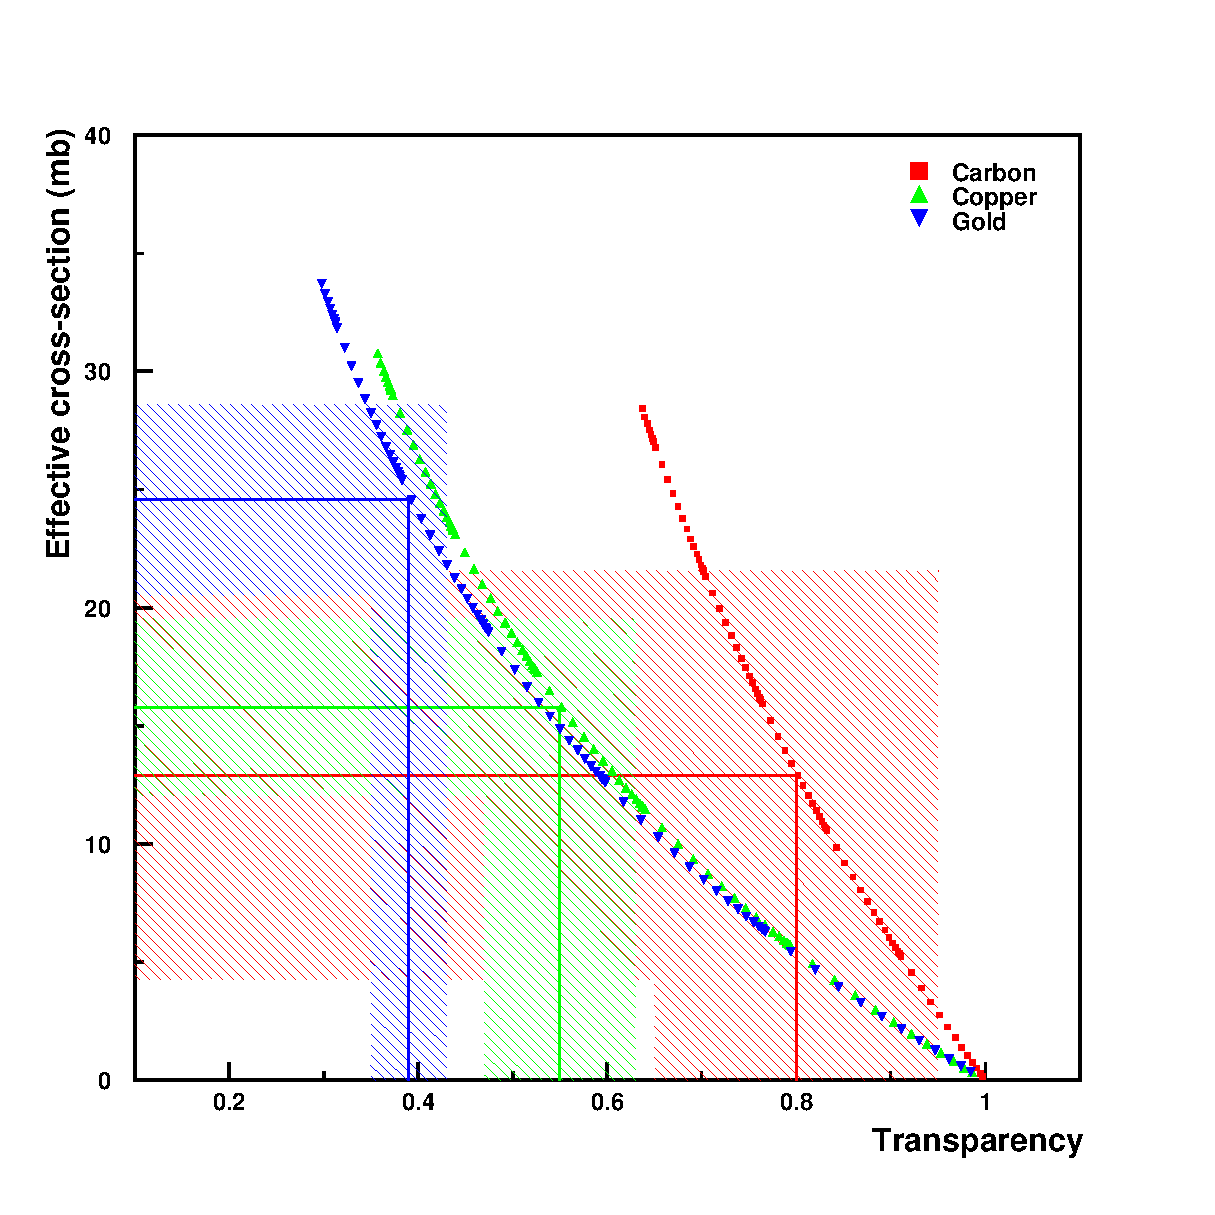
\includegraphics[width=0.8\columnwidth]{eff_t_all}
  \caption[Effective cross section comparison.]{\label{fig:eff_t_all}Effective cross section comparison.\\\\ Data points in RED are for carbon, GREEN data points are for copper and BLUE data points are for gold, considering only statistical uncertainty for kinematics1($Q^2$=1.1 $(\mathrm{GeV/c})^2$).}
\end{figure}
%\setlength{\figwidth}{0.8\linewidth}
%\Figure{eff_t_all}{\figwidth}{Effective cross section comparison. Data points in \textcolor{red}{RED} are for carbon, \textcolor{green}{GREEN} data points are for copper and \textcolor{blue}{BLUE} data points are for gold, considering only statistical uncertainty for kinematics1($Q^2$=1.1 $(\mathrm{GeV/c})^2$).}

The average effective cross section has been calculated for different kinematic settings by weighted average over different targets, as shown in Eq. \ref{equ:effective}. The average effective cross sections for $K^+$ are listed in \Tableref{eff_cr2} and shown in \figureref{eff_av_all} in BLUE.

\begin{equation} \label{equ:effective}
\sigma_{eff}^{av} = 
\frac{\left(1/\sigma_{err}^{C}\right)^{2}\sigma_{eff}^{C}+ \left(1/\sigma_{err}^{Cu}\right)^2\sigma_{eff}^{Cu}+
\left(1/\sigma_{err}^{Au}\right)^2\sigma_{eff}^{Au}}
{\left(1/\sigma_{err}^{C}\right)^2+ \left(1/\sigma_{err}^{Cu}\right)^2+\left(1/\sigma_{err}^{Au}\right)^2}
\end{equation}

\Table{eff_cr2}{Average effective cross section for different $Q^2$ for kaons.}

\begin{table}
  \caption[Effective cross section for different targets and of $Q^2$ for pion.]{\label{tab:eff_cr3}Effective cross section for different targets and of $Q^2$ for pion.}
\begin{center}
\begin{tabular}{||c|c|c|c|c||}\hline
 Target & $Q^2$ & $P_k$ & Transparency & Effective cross section \\
 & $(GeV/c)^2$ & $(GeV/c)$ & & (mb)\\\hline
Carbon & 1.1 & 2.8 & 0.67$\pm$0.01 &24.82$\pm$1.12 \\
Copper & 1.1 & 2.8 & 0.45$\pm$0.01 &22.34$\pm$0.75 \\
Gold   & 1.1 & 2.8 & 0.28$\pm$0.01 &35.99$\pm$1.38 \\\hline
Carbon & 2.2 & 3.2 & 0.65$\pm$0.01 &27.07$\pm$1.32 \\
Copper & 2.2 & 3.2 & 0.45$\pm$0.01 &22.34$\pm$0.75 \\
Gold   & 2.2 & 3.2 & 0.29$\pm$0.01 &34.73$\pm$1.34 \\\hline
Carbon & 3.0 & 3.4 & 0.68$\pm$0.02 &23.77$\pm$2.20 \\
Copper & 3.0 & 3.4 & 0.43$\pm$0.01 &23.83$\pm$0.66 \\
Gold   & 3.0 & 3.4 & 0.29$\pm$0.01 &34.73$\pm$1.34 \\\hline
Carbon & 3.9 & 4.1 & 0.77$\pm$0.02 &15.21$\pm$1.58 \\
Copper & 3.9 & 4.1 & 0.52$\pm$0.01 &17.56$\pm$0.48 \\
Gold   & 3.9 & 4.1 & 0.34$\pm$0.01 &28.84$\pm$0.98 \\\hline
Carbon & 4.7 & 4.4 & 0.70$\pm$0.03 &21.67$\pm$3.00 \\
Copper & 4.7 & 4.4 & 0.53$\pm$0.02 &17.20$\pm$1.21 \\
Gold   & 4.7 & 4.4 & 0.33$\pm$0.02 &30.23$\pm$1.38 \\\hline
\end{tabular}
\end{center}
\end{table}
%\Table{eff_cr3}{Effective cross section for different targets and of $Q^2$ for pion.}

\SubSection{Effective Cross Section of Pions ($\pi^+$)}%
%\label{Effective crorss-section of pions($\pi^+$)}
Applying the same technique used in section \ref{Effective cross-section of kaons($K^+$)}, we have calculated the effective $\pi^+$-nucleon cross section from the measured pion transparency \cite{BC06}. The effective cross sections for different targets for five kinematic settings of $Q^2$ = 1.1, 2.2, 3.0, 3.9 and 4.7 $(\mathrm{GeV/c})^2$ are shown in \Tableref{eff_cr3}. Average cross sections are listed in \Tableref{eff_cr4} and shown in \figureref{eff_av_all} in GREEN.

\Table{eff_cr4}{Average effective cross section for different $Q^2$ for pion.}

\begin{figure}[!tbp]
  \centering
  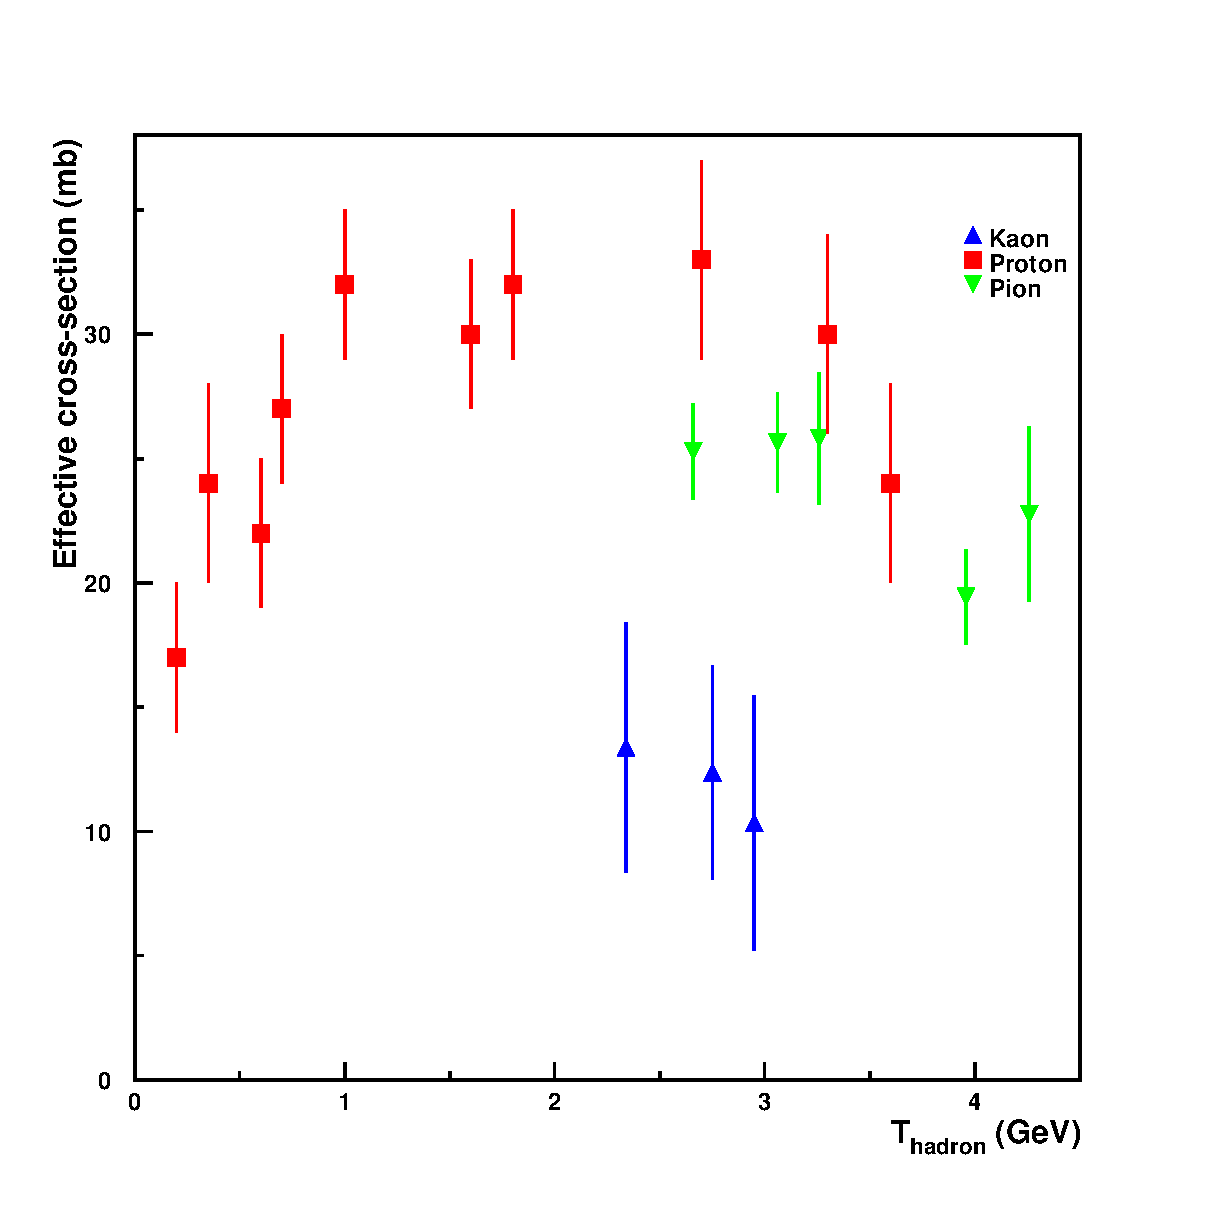
\includegraphics[width=0.8\columnwidth]{eff_av_all}
  \caption[Effective cross section vs transparency.]{\label{fig:eff_av_all}Effective cross section vs transparency.\\\\ Data points in RED is for protons, GREEN data points are for $\pi^+$ and BLUE data points are from this analysis for $K^+$, considering only statistical uncertainty \cite{hinton01}.}
\end{figure}
%\setlength{\figwidth}{0.8\linewidth}
%\Figure{eff_av_all}{\figwidth}{Effective cross section vs transparency. Data points in \textcolor{red}{RED} is for protons, \textcolor{green}{GREEN} data points are for $\pi^+$ and \textcolor{blue}{BLUE} data points are from this analysis for $K^+$, considering only statistical uncertainty \cite{hinton01}.}

\SubSection{Effective Cross Section of Protons (p)}%
\label{Effective cross-section of protons(p)}
The average effective cross section for different kinematic settings for protons are listed in \Tableref{eff_cr6} from reference\cite{carroll} and shown in \figureref{eff_av_all} by RED.

\Table{eff_cr6}{Average effective cross section for different $T_K$ for protons\cite{jlabp2}.}

\SubSection{Effective Cross Section for All Hadrons ($\pi^+$, $K^+$, p)}%
The world data \cite{PDG} on p-p, p-n total cross sections as a function of kinetic energy ($T_{hadron}$) was fitted to a function form as shown in \figureref{crr1}. The error bars are statistical only. $T_{hadron}$ is defined as 

\begin{equation} \label{equ:effective4}
T_{hadron} = \sqrt{P_{hadron}^2 + M_{hadron}^2} - M_{hadron}
\end{equation}

We also performed similar fits for the world $\pi^+$-p, $\pi^+$-n and $K^+$-p, $K^+$-n data as shown in \figureref{crr1}. We then compared the effective cross section extracted from our experiment to these fitted forms for the proton, pion and kaon. The results are shown in \figureref{crr2} with RED for protons, GREEN for pions and BLUE for kaons. 

%where $P_{hadron}$ and $M_{hadron}$ are the momentum and mass of the hadron respectively. Using this formula we have calculated the kinetic energy for kaons, pions and protons corresponding to different kinematic settings. The world data for p-p, p-n and n-n elastic scattering data were fited to compare with data and has been shown in the \figureref{crr1}. The error bar represent the ststistical uncertinity. In the \figureref{crr2} we have ploted the effective proton-nucleon cross section from 
%\Tableref{eff_cr6} for different kinematic settings with world data fit \cite{PDG} in \textcolor{red}{RED}. Similarly for pions and kaons are shown in \textcolor{green}{GREEN} and \textcolor{blue}{BLUE} respectively.
\Table{scalefactor}{Scale factors for different hadron-nucleon scattering.}

Note that the world data of hadron-nucleon scattering cross sections are obtained from hadron scattering experiments. In this analysis, we compared the electron scattering effective cross section with those obtained from hadron-scattering experiments.

The scale factors in \Tableref{scalefactor} indicate the differences in the nature of the probes used: electromagnetic for electrons vs strong for hadrons. Since the electromagnetic interaction is weaker than the strong interaction, hence electrons can probe deeper into the nucleus compare to hadrons. This leads the scale factors between electron-scattering and hadron-scattering technique. The remarkable agreement between the K.E. dependence of the proton cross sections obtained from electron scattering and hadron scattering point to the similar reaction mechanisms that are well described within traditional nuclear physics. The deviation of the pion results indicate a break down of traditional nuclear physics reaction mechanisms for pions. For the kaons, our uncertainties are too large to draw any conclusions.

\begin{figure}[!tbp]
  \centering
  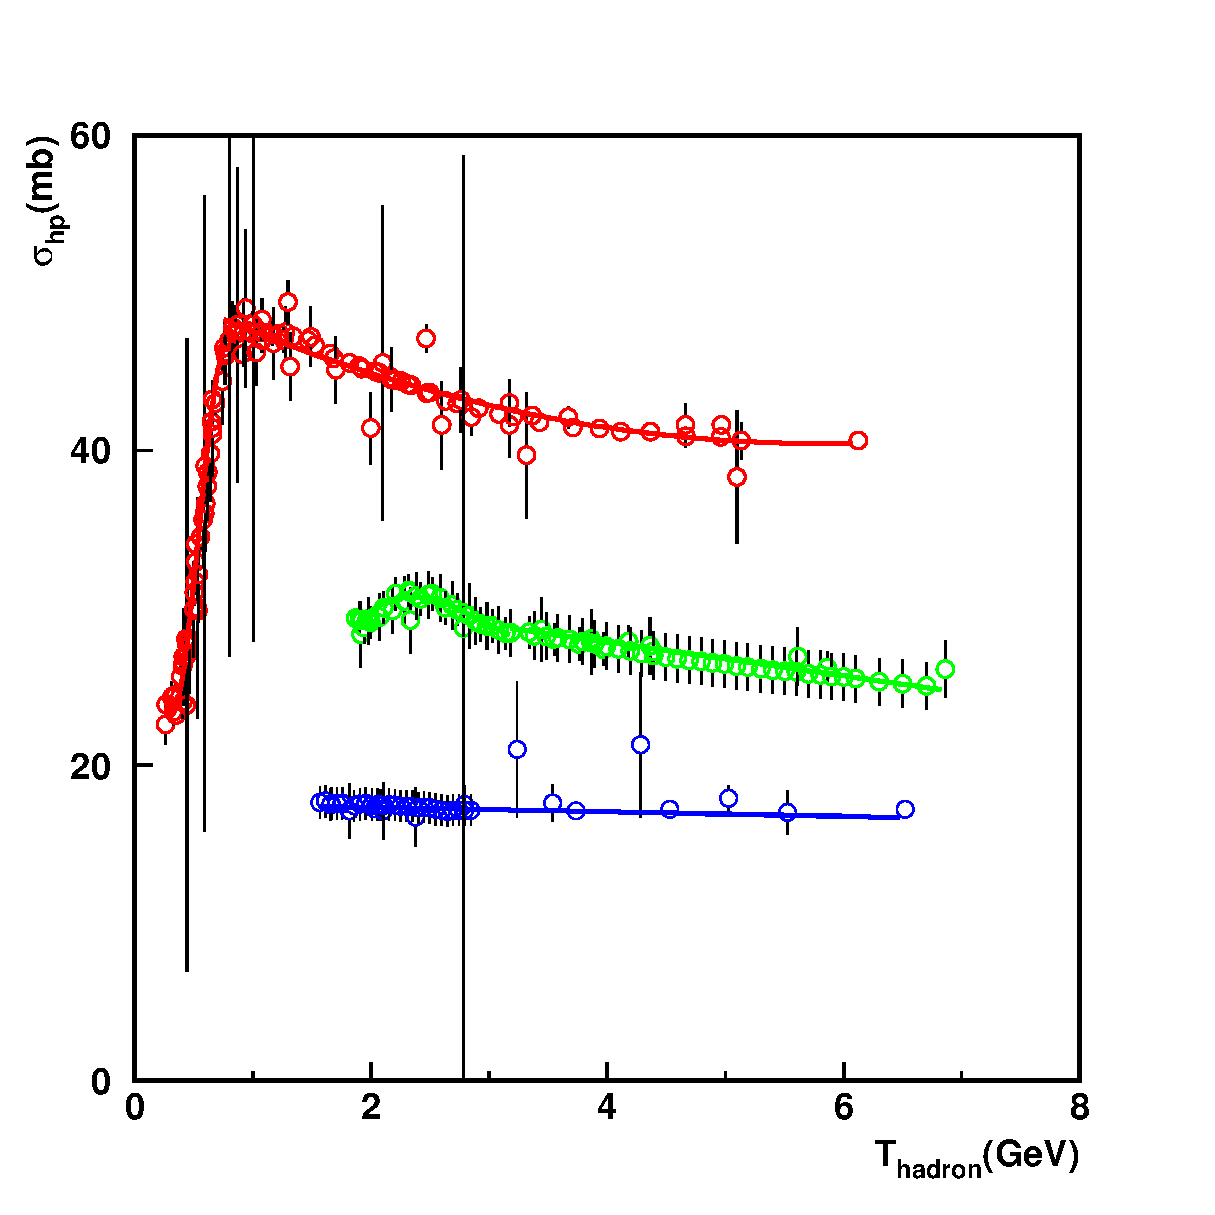
\includegraphics[width=0.8\columnwidth]{crr1}
  \caption[Hadron-proton total cross section vs $T_{hadron}$.]{\label{fig:crr1}Hadron-proton total cross section vs $T_{hadron}$.\\\\ Data points in RED are for protons, GREEN data points are for $\pi^+$ and BLUE data points are from this analysis for $K^+$ from \cite{hinton01}.}
\end{figure}
%\setlength{\figwidth}{0.8\linewidth}
%\Figure{crr1}{\figwidth}{Hadron-proton total cross section vs $T_{hadron}$: Data points in \textcolor{red}{RED} are for protons, \textcolor{green}{GREEN} data points are for $\pi^+$ and \textcolor{blue}{BLUE} data points are from this analysis for $K^+$ from \cite{hinton01}.} 

\begin{figure}[!tbp]
  \centering
  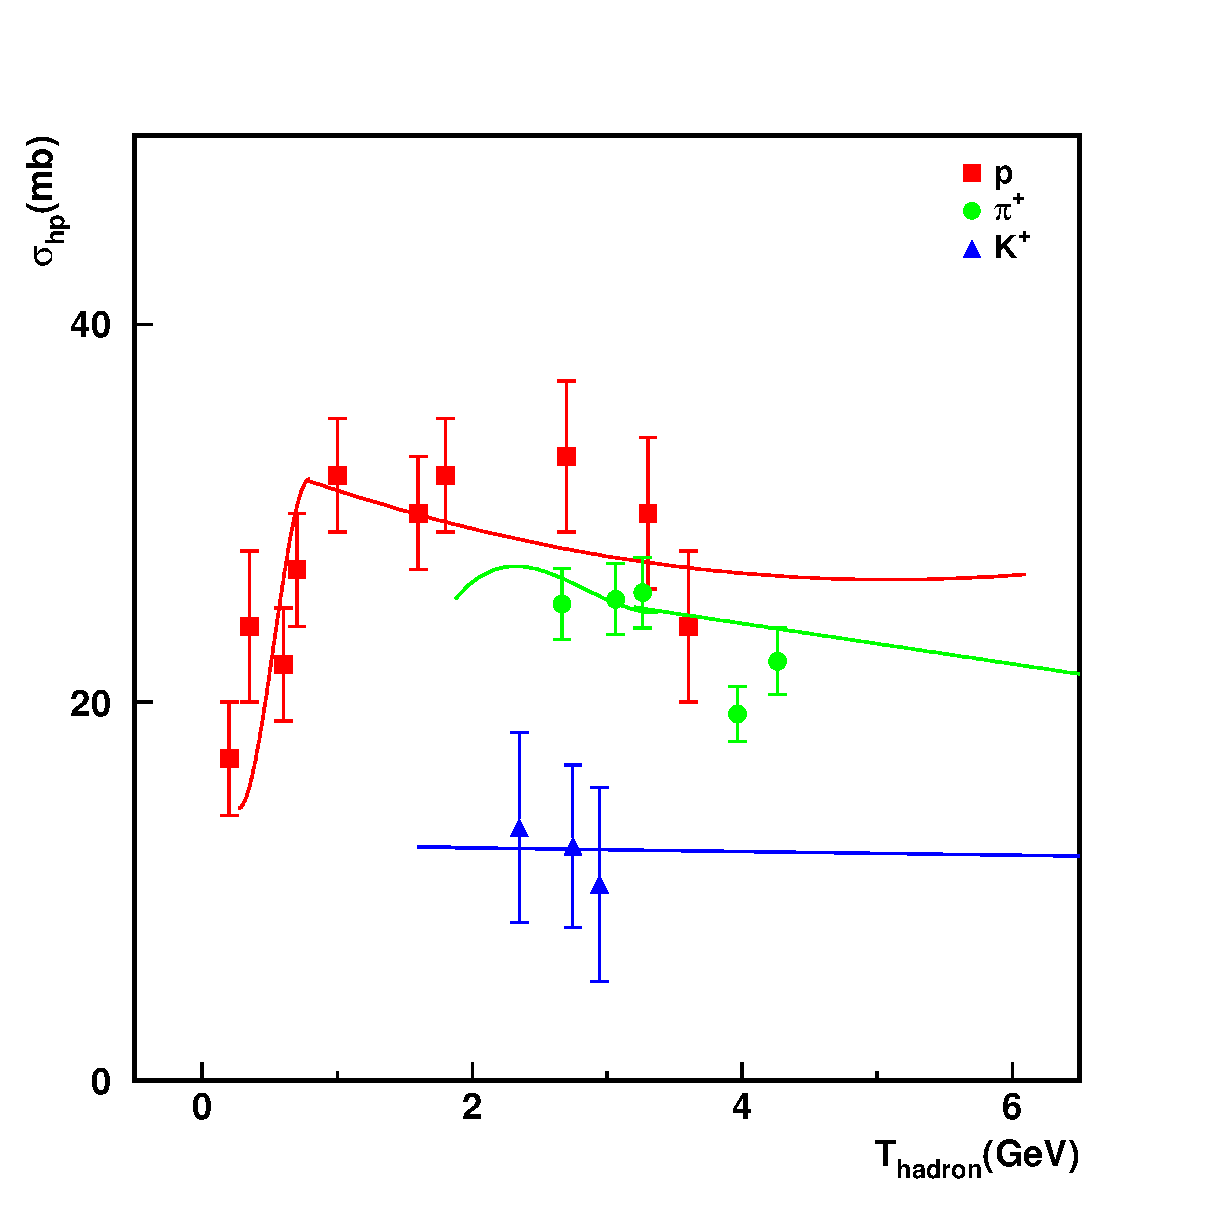
\includegraphics[width=0.8\columnwidth]{crr2}
  \caption[Comparison of effective and hadron-proton total cross section.]{\label{fig:crr2}Comparison of effective and hadron-proton total cross section.\\\\ Data points in RED are for protons from \cite{hinton01}, GREEN data points are for $\pi^+$ and BLUE data points are from this analysis for $K^+$. The fits are from hadron-scattering world data\cite{PDG} with scale factors given in \Tableref{scalefactor}.}
\end{figure}
%\setlength{\figwidth}{0.8\linewidth}
%\Figure{crr2}{\figwidth}{Effective cross section vs $T_{hadron}$: Data points in \textcolor{red}{RED} are for protons from \cite{hinton01}, \textcolor{green}{GREEN} data points are for $\pi^+$ and \textcolor{blue}{BLUE} data points are from this analysis for $K^+$. The fits are from hadron-scattering world data\cite{PDG} with scale factors given in \Tableref{scalefactor}.} 

\SubSection{$A$ Dependency of Transparency}%
The $A$ dependence of the nuclear transparency is extracted from the simple ansatz $T = A^{1 - \alpha}$, where $\alpha$ is used to parametrize the nuclear cross section and $\sigma_N$ is in terms of the elementary nucleon cross-section, $\sigma_{0}$ as $\sigma_N = \sigma_0A^{\alpha}$.

%From the observation what we found is kaon is mostly transparent.
\begin{table}
  \caption[$\alpha$ values for different $Q^2$ for kaons with respect to $LD_2$.]{\label{tab:alpha2}$\alpha$ values for different $Q^2$ for kaons with respect to $LD_2$.}
\begin{center}
%\centering
\begin{tabular}{||c|c|c||}\hline
 Kinematics & $Q^2$ & $\alpha$ \\
 & $(GeV/c)^2$ & \\\hline
Kin1 & 1.1 &0.84$\pm$0.06 \\
Kin2 & 2.2 &0.91$\pm$0.04 \\
Kin3 & 3.0 &0.92$\pm$0.05 \\\hline
\end{tabular}
\vspace{-0.5cm}
\end{center}
\end{table}
%\Table{alpha2}{$\alpha$ values for different $Q^2$ for kaons with respect to $LD_2$.}

The $Q^2$ dependence of nuclear transparency was very small for the kinematics range of $Q^2$= 1.1 $(\mathrm{GeV/c})^2$ to $Q^2$= 3.0 $(\mathrm{GeV/c})^2$. Fitting the transparency for a particular $Q^2$ to T = $A^{1-\alpha}$, we get $\alpha$ as shown in \Tableref{alpha2}.\footnote{The value of $\alpha$ with respect to hydrogen is given in APPENDIX A, \Tableref{alpha1}.} We extracted transparency and effective cross section for different kinematic settings for kaons in this analysis and calculated effective cross sections for available transparencies for protons and pions. $\alpha$ values have been plotted against effective cross section from this work and reference \cite{jlabp2} in \figureref{carolplot}.

\begin{figure}[!tbp]
  \centering
  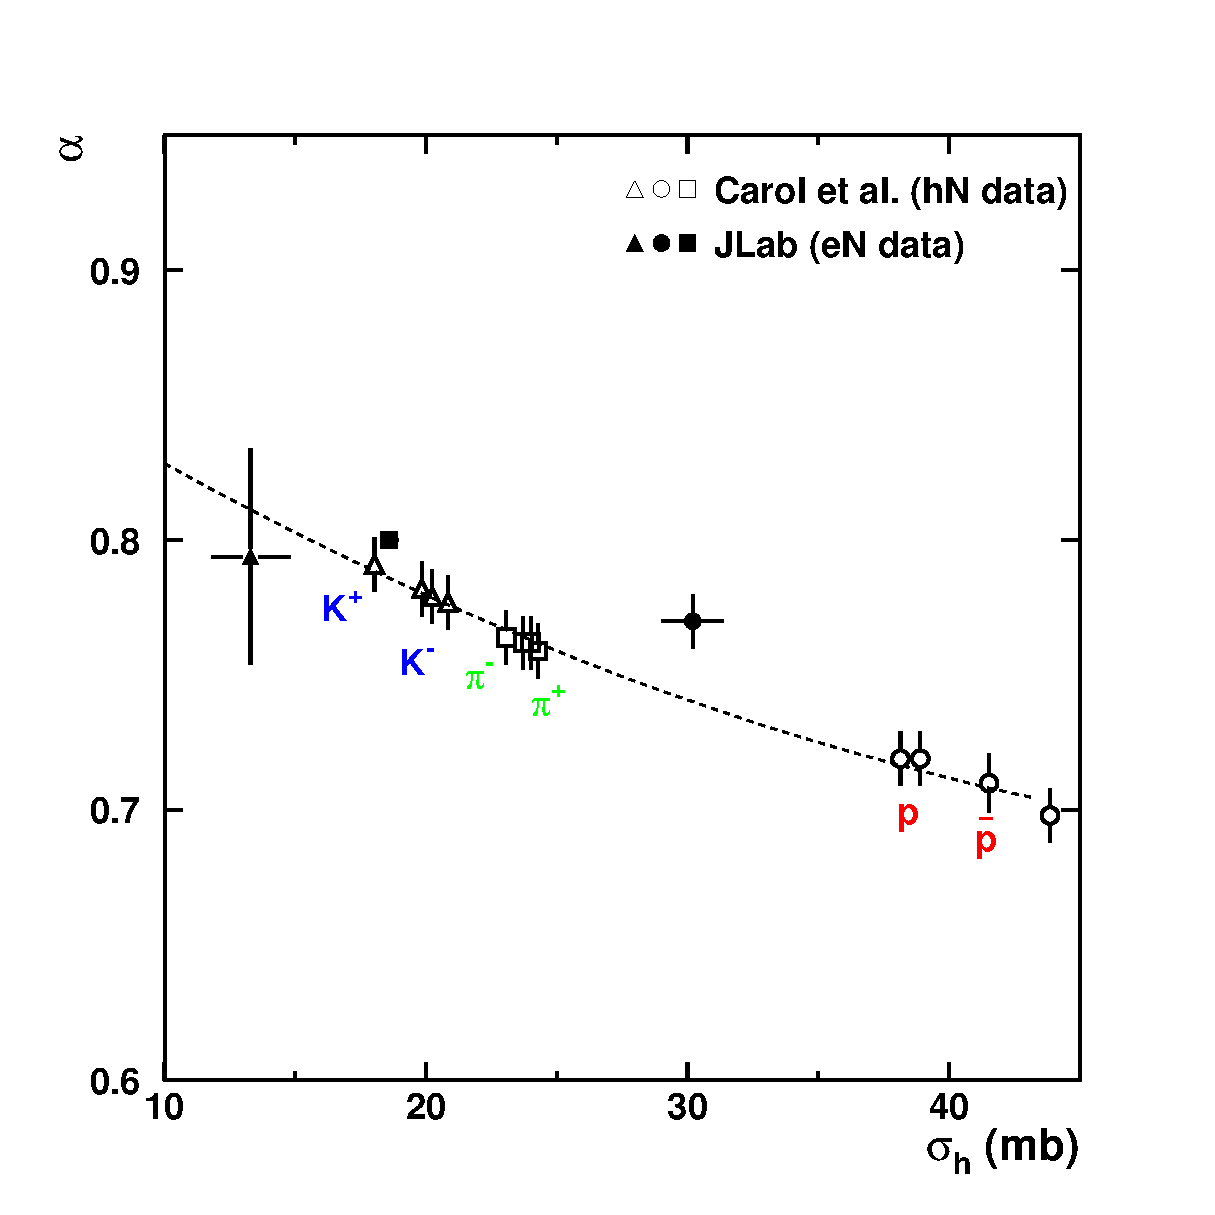
\includegraphics[width=0.8\columnwidth]{carolplot}
  \caption[$\alpha$ from electro-production of hadrons and from hadron-scattering.]{\label{fig:carolplot}$\alpha$ from electro-production of hadrons and from hadron-scattering.\\\\ $\alpha$ from electro-production of kaons (from this analysis), pions, and protons are shown by solid triangle, square, and cicrle, respectively. Similarly, $\alpha$ from hadron-scattering reactions are shown by empty points and fitted with dotted curve \cite{carroll}.}
\end{figure}
%\setlength{\figwidth}{0.8\linewidth}
%\Figure{carolplot}{\figwidth}{$\alpha$ from electro-production of kaons (from this analysis), pions, and protons are shown by solid triangle, square, and cicrle, respectively. Similarly, $\alpha$ from hadron-scattering reactions are shown by empty points and fitted with dotted curve \cite{carroll}.}

The results indicate that the effective cross section obtained from electron-scattering is smaller than hadron-scattering (as expected from the nature of the probe). For protons and pions, the parameter $\alpha$ extracted from electro-production measurements do not agree with those obtained from hadro-production, some of these differences may also be related to the strength of the interaction between the incident hadron and the nucleons. For kaons, the parameter $\alpha$ from electro-production is consistent within statistical uncertainties, with those obtained from hadro-production. However, due to the low statistics of kaons in our data set, we cannot draw any strong conclusions.
%The results indicate that not only the effective cross section obtained from electron-scattering is smaller than hadron-scattering (as expected from the nature of the probe). For protons and pions, $\alpha$ extracted from electro-production  measurements do not agree with those obtained from hadro-production but for kaons, the $\alpha$ are consistent within statistical uncertainties. Due to low statistics of kaons in our data set, our results do not draw any strong conclusions. 